\section{Summary of Contributions}

This project successfully demonstrates the integration of artificial intelligence, machine learning, and full-stack web development to create a functional, user-centric AI-Based Trip Planner Web Application. By addressing the cognitive overload and computational complexity inherent in travel planning, the system provides a seamless end-to-end pipeline from user constraints to fully structured itineraries. The key contributions of this work are summarized and detailed below.

\subsection{Intelligent Destination Recommendation System}

The project develops and deploys a machine learning-based destination recommendation engine using the \textbf{Decision Tree Classifier} from Scikit-learn \cite{pedregosa2011}. The system accepts user-specified travel constraints (budget, days, climate, travel type) and predicts the most suitable travel destination from a curated list of 36 Indian destinations.
The design of this system includes several technical highlights:
\begin{itemize}
    \item \textbf{Synthetic Dataset Engineering}: Due to the lack of publicly available, structured datasets mapping user constraints directly to specific Indian travel destinations, a custom synthetic dataset of 1,000 samples was engineered. This dataset features mathematically distinct boundaries to model user preferences.
    \item \textbf{Feature Optimization and Bijective Encoding}: The inputs—budget, duration of stay, preferred climate (hot, cold, moderate), and travel type (adventure, family, leisure, spiritual)—are transformed using optimized LabelEncoders. These transformations are verified to be bijective, preventing any information loss during preprocessing.
    \item \textbf{Hyperparameter Tuning}: Through grid search validation, a maximum depth of 8 was chosen. This prevents overfitting while ensuring that all 36 destinations can be successfully mapped.
    \item \textbf{Efficient Deserialization}: The trained model is serialized using Joblib. This allows the Django backend to perform real-time inference in less than 5 milliseconds, enabling responsive user experiences.
\end{itemize}

\subsection{Dynamic Itinerary Generation}

The application implements an automated itinerary generation system that produces structured, day-wise travel schedules following destination prediction. Rather than displaying static travel advice, the engine dynamically adapts schedules to match the user's specified trip duration and budget.
The mechanics of the dynamic generator include:
\begin{itemize}
    \item \textbf{Dynamic Day Allocation}: The itinerary generator distributes activities dynamically based on the number of days specified by the user. It constructs a complete daily cycle consisting of morning, afternoon, and evening activities.
    \item \textbf{Granular Cost Distribution Model}: The total user-defined budget is distributed across four critical travel cost categories using structured proportions: 40\% for accommodation, 25\% for food, 20\% for transportation, and 15\% for activities. This ensures that the generated cost breakdown matches the total budget exactly.
    \item \textbf{JSON-Structured Data Delivery}: The backend generates structured JSON output mapping day numbers, category costs, and activities. This structure allows the client-side JavaScript to render interactive, tabbed schedules without page reloads.
\end{itemize}

\subsection{Full-Stack Web Application Development}

The complete web application is built using \textbf{Django} \cite{django2026} following the Model-View-Template (MVT) architectural pattern. The backend architecture supports high modularity and secure data flow:
\begin{itemize}
    \item \textbf{Secure Authentication}: Employs a custom user model extending Django's built-in \texttt{AbstractUser} system, allowing future scalability of user profile attributes. Password hashing (PBKDF2) and secure session management are active across all protected routes.
    \item \textbf{RESTful API Architecture}: Implemented with Django REST Framework (DRF), exposing clean endpoints for recommendation requests and user trip management.
    \item \textbf{Robust Database Schema}: Designed using Django ORM mapping user accounts, active trips, and deleted trips with relational constraints on a SQLite3 database.
    \item \textbf{Middleware and Security Headers}: Integration of CSRF protection, clickjacking protection, and XSS filtering across all templates.
\end{itemize}

\subsection{User-Centric Features}

The system provides personalized trip management capabilities that enhance user experience:
\begin{itemize}
    \item \textbf{Interactive User Dashboard}: A central hub displaying saved trip plans using clean tabular layouts, including destination metadata, costs, and high-quality images.
    \item \textbf{Stateful Soft-Delete Mechanism}: Rather than permanently deleting records, which leads to accidental data loss, the application implements a soft-delete mechanism. Trips are flagged using an \texttt{is\_deleted} boolean field and stored in a recovery trash bin.
    \item \textbf{One-Click Restoration}: Users can review soft-deleted trips and restore them back to their active dashboard in a single action, updating the database state immediately.
    \item \textbf{Fluid and Responsive Styling}: Styled with Vanilla CSS using CSS Grid and Flexbox layouts. This guarantees cross-device compatibility, offering an equally premium experience on mobile viewports, tablets, and wide-screen desktops.
\end{itemize}

\subsection{Real-World Applicability}

The application demonstrates practical applicability for Indian travel planning:
\begin{itemize}
    \item \textbf{Diverse Destination Coverage}: Covers 36 distinct Indian destinations spanning across multiple geographical regions (hilly, coastal, historical, and metropolitan).
    \item \textbf{Realistic Financial Modeling}: Uses Indian Rupee (INR) budget brackets that align with real-world Indian tourism costs, split by low, medium, and high-end budgets.
    \item \textbf{Cultural Relevance}: Incorporates localized activity recommendations (e.g., houseboats in Alleppey, temple visits in Varanasi, trekking in Manali) that reflect the specific travel characteristics of the Indian subcontinent.
\end{itemize}

\section{Critical Analysis and Limitations}

Although the developed prototype successfully meets all initial functional requirements, a critical academic evaluation reveals several inherent limitations that must be acknowledged:

\begin{itemize}
    \item \textbf{Reliance on Synthetic Training Data}: Due to privacy constraints and the lack of public datasets mapping user demographics to Indian destinations, the Decision Tree model was trained on synthetic data. While this data possesses clear mathematical boundaries, it may not fully capture the chaotic, non-linear preferences of real-world travelers.
    \item \textbf{Static Offline Recommendations}: The recommendation model is trained offline and serialized. Once deployed, it does not dynamically update based on new user feedback or evolving travel trends unless manually retrained and redeployed.
    \item \textbf{Lack of Real-Time Pricing}: The financial calculations rely on static percentage allocations. They do not account for real-world market dynamics such as seasonal price surges, high-demand hotel occupancy rates during festivals, or real-time flight price changes.
    \item \textbf{Single-Destination Constraints}: The itinerary generator assumes a single destination per trip. The system cannot currently generate multi-city travel routes or optimize paths spanning across multiple states in a single query.
    \item \textbf{Limited Feature Vector}: The input vector contains only four primary constraints. Demographics such as age, accessibility requirements, dietary preferences, and travel company size (e.g., solo traveler vs. group) are not factored into the model.
\end{itemize}

\section{Future Enhancements}

To address these limitations and expand the application's commercial utility, several future enhancements have been designed:

\subsection{Global Dataset Expansion}

The current dataset covers 36 Indian travel destinations. Future work includes expanding the recommendation system to cover international destinations.

\begin{figure}[H]
    \centering
    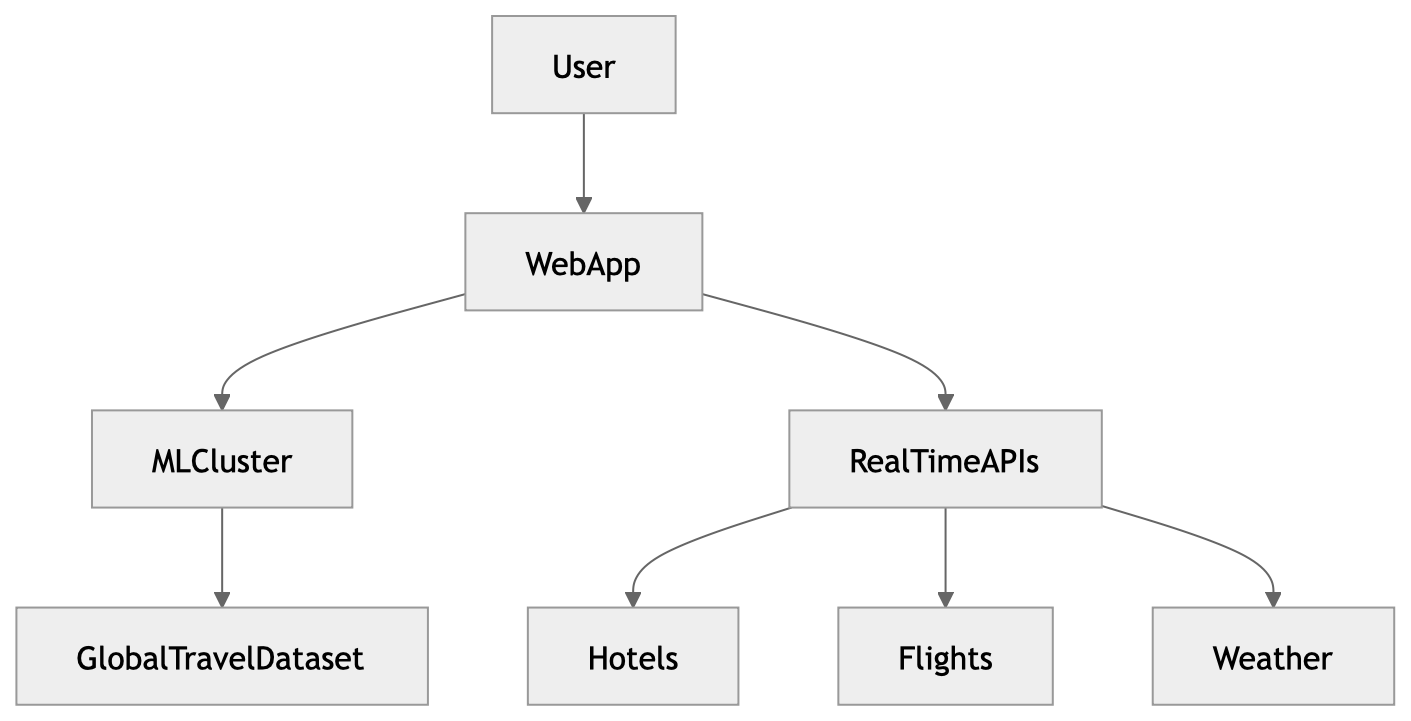
\includegraphics[width=0.9\textwidth,height=0.7\textheight,keepaspectratio]{images/Future Scalable Architecture.png}
    \caption{Future Scalable Architecture}
    \label{fig:future-architecture}
\end{figure}

Expanding the scale of the destination dataset will require:
\begin{itemize}
    \item \textbf{Global Data Scraping and Consolidation}: Developing web scrapers to gather destination metadata from tourism portals (e.g., TripAdvisor) and combining them with large-scale Kaggle datasets.
    \item \textbf{Dynamic Currency Conversion}: Integrating exchange rate APIs to support international budgeting, converting costs seamlessly between INR, USD, EUR, and other global currencies.
    \item \textbf{Localization and Multilingual Support}: Utilizing internationalization (i18n) frameworks to translate itineraries and descriptions into regional and foreign languages.
    \item \textbf{Visa and Regulation Parsing}: Automatically extracting visa requirements and travel advisory levels based on the user's nationality and destination country.
\end{itemize}

\subsection{Real-Time Price API Integration}

The current system uses static budget ranges. Future enhancements will incorporate real-time price data through third-party API integrations, turning the application into a live travel booking aggregator:
\begin{itemize}
    \item \textbf{GDS and Flight API Connections}: Connecting to Amadeus or Skyscanner APIs to retrieve real-time flight costs and display booking links based on the user's selected trip dates.
    \item \textbf{Hotel Booking Integrations}: Fetching live accommodation rates using Booking.com or Expedia APIs to replace static budget estimations with real-time hotel prices.
    \item \textbf{Dynamic Activity Booking}: Integrating with local tour operator APIs (e.g., Klook, GetYourGuide) to allow users to book activities directly from their generated itineraries.
    \item \textbf{Local Weather Mapping}: Querying the OpenWeatherMap API during the trip dates to display active weather warnings or packing suggestions.
\end{itemize}

\subsection{Collaborative Filtering Recommendations}

The current recommendation engine uses a supervised classification approach. Future work will explore hybrid recommendation models combining content-based features with collaborative filtering:
\begin{itemize}
    \item \textbf{User-Item Interaction Matrix}: Building a system to record user actions (views, saves, deletes, and clicks) to populate a sparse interaction matrix.
    \item \textbf{Matrix Factorization (SVD)}: Implementing Singular Value Decomposition to uncover latent preferences and recommend destinations that similar users enjoyed.
    \item \textbf{Neural Collaborative Filtering (NCF)}: Designing deep learning models to learn complex, non-linear user-destination interactions, bypassing the limitations of shallow classifiers.
    \item \textbf{Addressing Cold Start}: Utilizing the existing Decision Tree model for new users, then transitioning them to collaborative filtering once sufficient history is gathered.
\end{itemize}

\subsection{Export and Sharing Features}

Future versions of the application will include trip plan export and social sharing capabilities to enhance viral marketing and user utility:
\begin{itemize}
    \item \textbf{High-Fidelity PDF Generation}: Integrating ReportLab or WeasyPrint to allow users to download clean, printable PDF brochures of their day-wise itineraries.
    \item \textbf{Automated Email Delivery}: Utilizing Django's email backend to send a copy of the itinerary directly to the user's inbox upon request.
    \item \textbf{Calendar Synchronization}: Providing ICS file exports and direct Google Calendar integration to block out itinerary activities in the user's personal calendar.
    \item \textbf{Social Sharing Extensions}: Implementing web share widgets with Open Graph meta tags to enable seamless sharing on platforms like WhatsApp, Twitter, and Instagram.
\end{itemize}

\subsection{Progressive Web Application (PWA) Support}

Converting the web application into a Progressive Web Application will extend its reach to mobile users without requiring native app development:
\begin{itemize}
    \item \textbf{Offline Itinerary Storage}: Implementing service workers to cache previously saved trips and destination images, allowing users to access itineraries even without internet connectivity (crucial when traveling in low-signal areas).
    \item \textbf{Local IndexedDB Integration}: Storing user input locally and syncing with the server once an internet connection is re-established.
    \item \textbf{Push Notifications}: Triggering alerts on the user's mobile device for travel checklist reminders or changes in flight schedules.
    \item \textbf{Home Screen Additions}: Configuring web app manifests to allow installing the application directly onto Android and iOS home screens with a native look and feel.
\end{itemize}

\section{Concluding Remarks}

The AI-Based Trip Planner Web Application bridges the gap between machine learning intelligence and full-stack web utility. By automating the destination prediction process based on personal constraints and creating structured daily plans, the system offers a viable prototype for the future of personalized tourism. The architecture laid out in this work—separating model training, API serialization, and stateful database management—serves as a scalable foundation. As travel environments shift towards real-time customization, the integration of collaborative networks and dynamic APIs will position this system as an indispensable, intelligent companion for travelers worldwide.
